\documentclass[unicode,10pt]{beamer}
\usetheme{ttiposter}

\usepackage{luatexja}
\usepackage{luatexja-fontspec}
\usepackage{geometry}
\usepackage{graphicx}
\usepackage{multicol}
\usepackage{subcaption}
\captionsetup{compatibility=false}

\setmainjfont{ipagp.otf}
\beamertemplatenavigationsymbolsempty

\geometry{a4paper,portrait,left=2truemm,width=206truemm,right=2truemm}
\newlength{\mycolumnwidth}
\setlength{\mycolumnwidth}{0.495\textwidth}
\newlength{\mytitlefigureheight}
\setlength{\mytitlefigureheight}{1.5em}

\newcommand{\arrow}{\textcolor{ttiblue}{\textbf{→}}\hspace{1ex}}
\newcommand{\itemtitle}[1]{#1\\}
\newcommand{\fire}[1]{\textcolor{red}{\textbf{#1}}}
\newcommand{\doublecolumns}[4]{
    \begin{minipage}[t]{#1}
      #2
    \end{minipage}
    \begin{minipage}[t]{#3}
      #4
    \end{minipage}}

\title{レーティング予測によるフォントを基盤としたレビュー解析}
\institute{豊田工業大学 知能数理研究室}
\author{外山 洋太, 三輪 誠, 佐々木 裕}
\date{\today}


\begin{document}
\begin{frame}[t]
\vspace{-1em} % HACK

\begin{columns}[onlytextwidth,t]
  \begin{column}{1.1\mycolumnwidth}
    \begin{block}{背景と目的}
      \begin{itemize}
        \item 対象タスク:表意、表語文字を含む言語におけるレーティング予測
        \item 応用例:企業における文書からの商品の評判分析
        \item 目的:文字の表層情報を利用したレーティング予測の実現
      \end{itemize}
    \end{block}
    \begin{figure}
      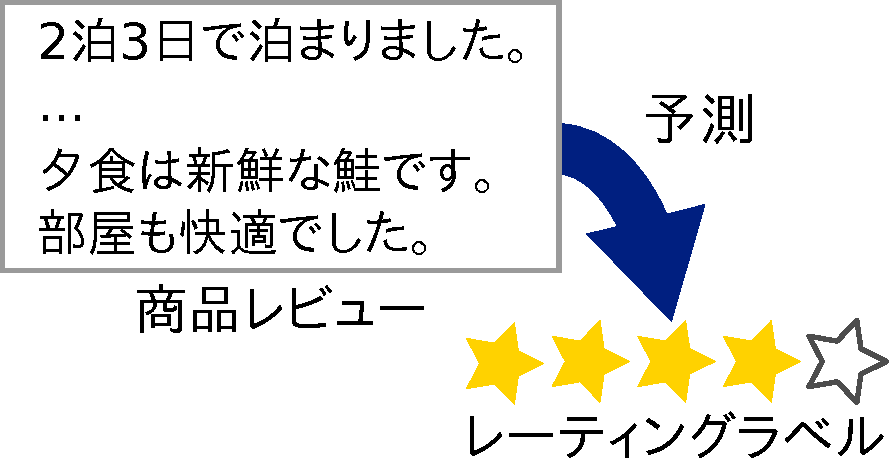
\includegraphics[width=0.7\linewidth]{fig/review.pdf}
    \end{figure}
  \end{column}
  \begin{column}{0.9\mycolumnwidth}
    \begin{block}{関連研究}
      \begin{itemize}
        \item \itemtitle{Hierarchical Attention Network (HAN) \cite{yang16}}
          \begin{itemize}
            \item Attention構造付きのRecurrent Neural Networkを用いた
                  文書分類モデル
            \item 文字または単語から文、文書までの階層的構造を利用
          \end{itemize}
          \arrow \fire{文字の表層情報の利用ができていない}
        \item \itemtitle{Radical-Enhanced Chinese Character Embedding
                         \cite{sun14}}
          \begin{itemize}
            \item 漢字-部首辞書を利用した漢字埋め込みの生成手法
            \item 対象タスクと漢字の部首当てについて同時に学習
          \end{itemize}
          \arrow \fire{漢字-部首辞書が余分に必要}
      \end{itemize}
    \end{block}
  \end{column}
\end{columns}


\begin{columns}[onlytextwidth,t]
  \begin{column}{\mycolumnwidth}
    \begin{block}{提案手法}
      \begin{itemize}
        \item 入力:フォント画像で表現されたレビュー
        \item 出力:予測したレーティングラベル
        \item 特徴
          \begin{itemize}
            \item \fire{フォント画像}から文字の意味情報を抽出
            \item HAN\cite{yang16}の手法を基に文字からの文書の階層構造を利用
          \end{itemize}
        \item 予測手順
          \begin{enumerate}
            \item foo
            \item bar
          \end{enumerate}
      \end{itemize}
      \begin{figure}
        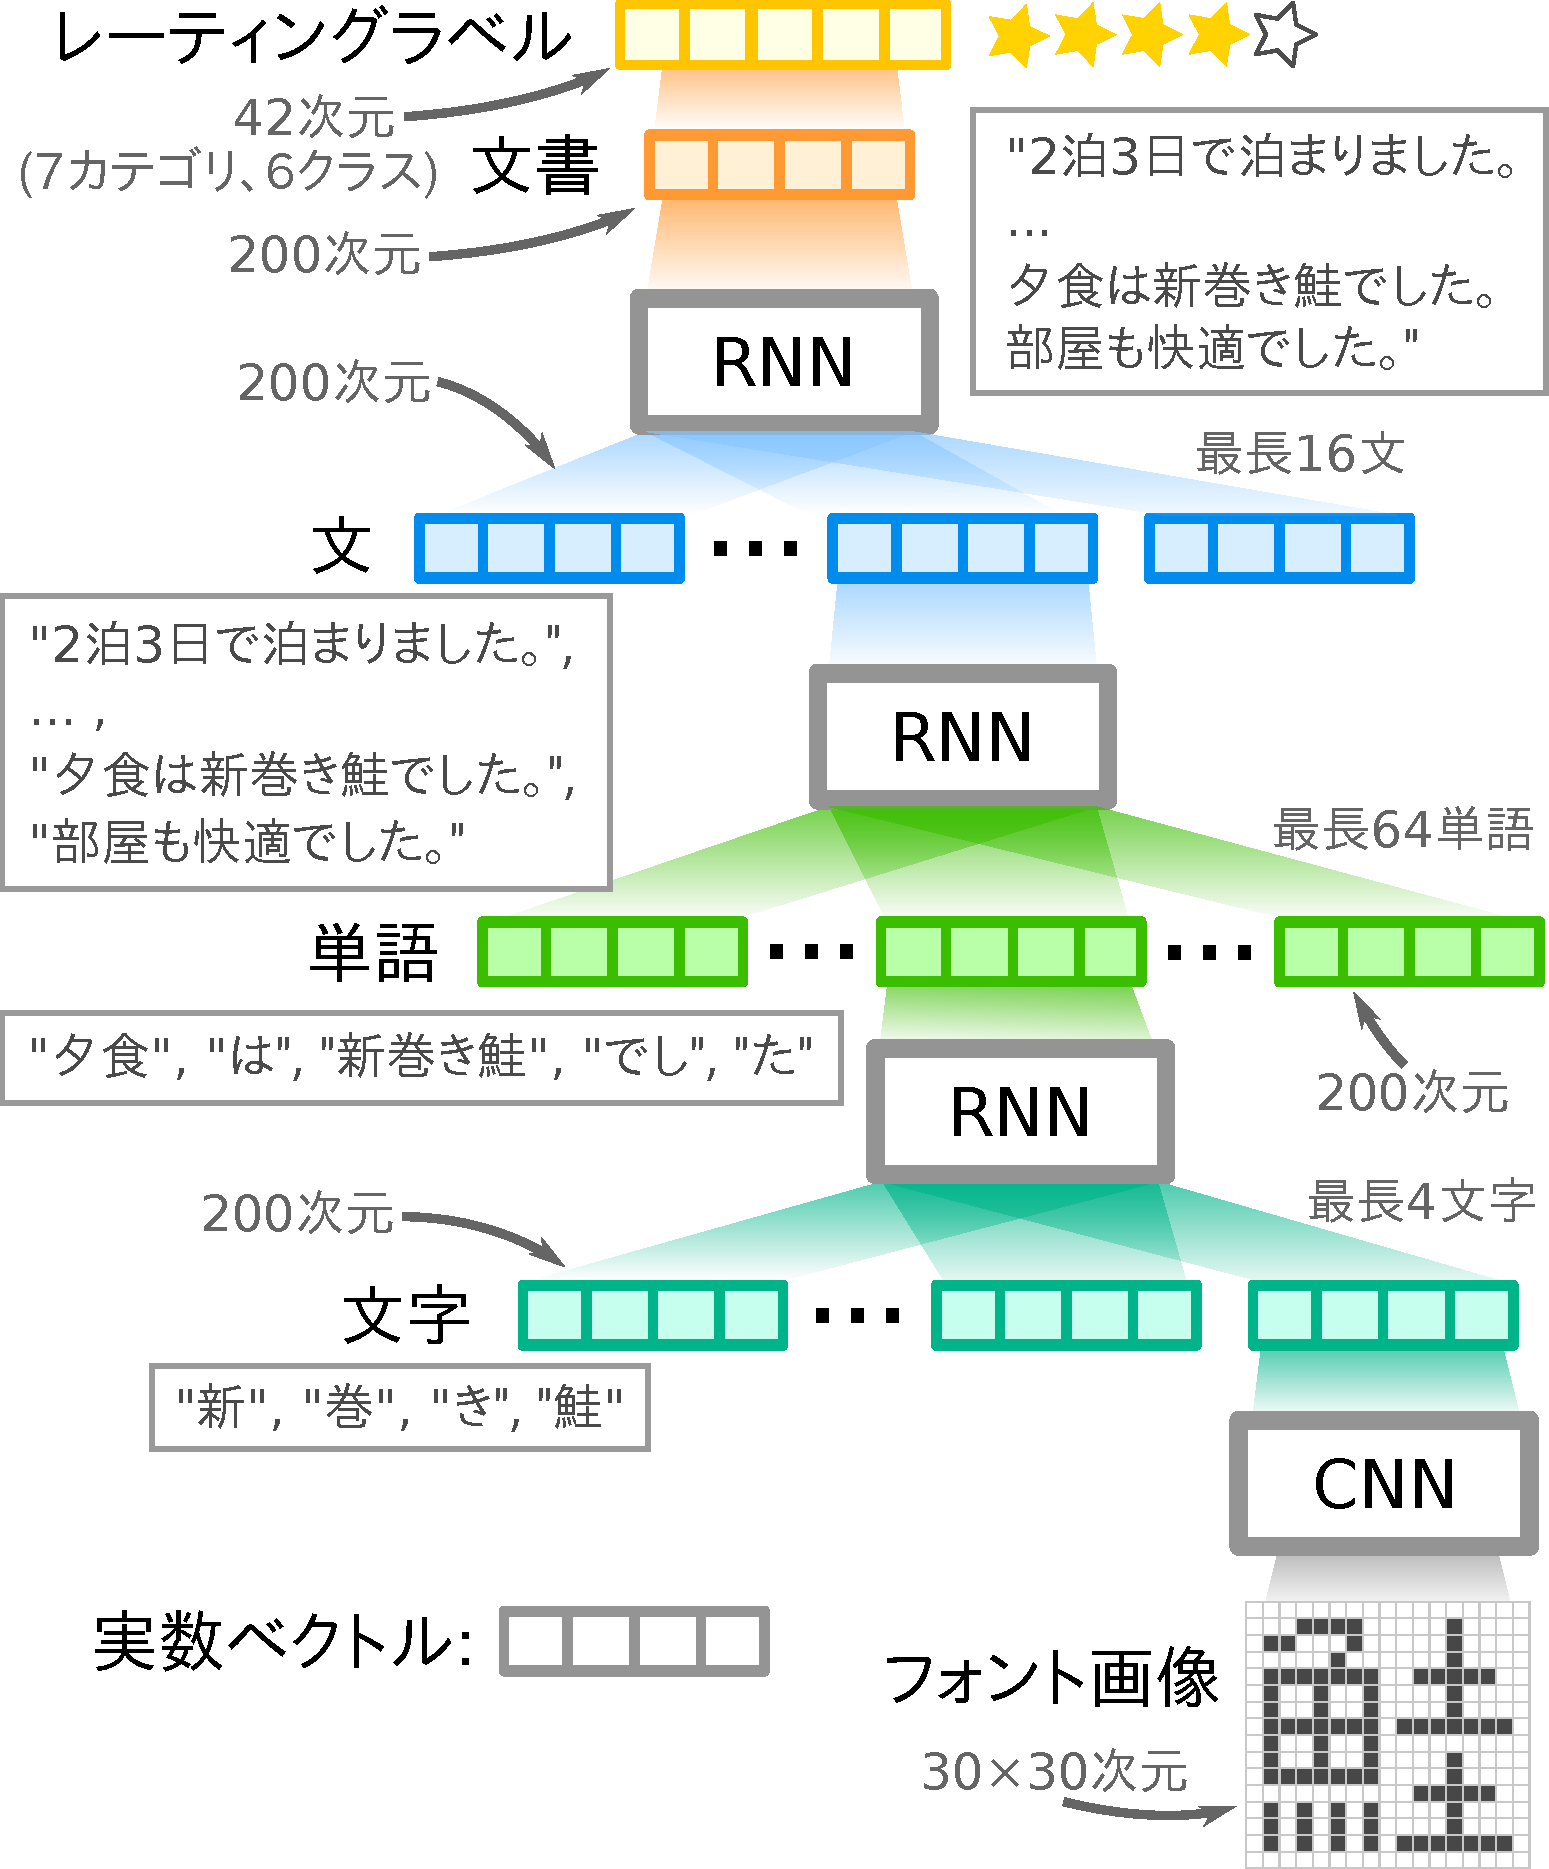
\includegraphics[width=0.8\linewidth]{fig/fcwsd.pdf}
      \end{figure}
    \end{block}
  \end{column}

  \begin{column}{\mycolumnwidth}
    \begin{block}{実験}
      \begin{itemize}
        \item \itemtitle{実験設定}
          \begin{itemize}
            \item 7カテゴリにおける0〜5点のレーティング予測の正答率を測定
            \item データセット:楽天トラベルのレビュー約330,000件
          \end{itemize}
      \end{itemize}

      \begin{itemize}
        \item \itemtitle{結果}
          \begin{itemize}
            \item 提案手法の従来手法より\fire{高い正答率}
          \end{itemize}
      \end{itemize}

      \begin{table}
        \centering
        \begin{tabular}{l | r r}
          手法 & 正答率 & RMSE \\
          \hline
          HAN \cite{yang16} & 0.483 & 0.81 \\
          提案手法 & \fire{0.503} & \fire{0.73} \\
        \end{tabular}
      \end{table}
    \end{block}

    \begin{block}{まとめ}
      \begin{itemize}
        \item フォント画像を用いたレーティング予測及びレビュー解析の手法を提案
        \item 提案手法による従来手法\cite{yang16}より高い正答率
        \item アテンションの可視化により
        \item \itemtitle{今後の予定}
          \begin{itemize}
            \item 可視化の方法を洗練
          \end{itemize}
      \end{itemize}
    \end{block}

    参考文献
    \bibliographystyle{jplain}
    \begin{thebibliography}{9}
      \bibitem{yang16}
        Zichao Yang et al.,
        Hierarchical Attention Networks for Document Classification.
        NAACL 2016, 2016.
      \bibitem{sun14}
        Yaming Sun et al.,
        Radical-Enhanced Chinese Character Embedding.
        ICONIP 2014, 2014.
    \end{thebibliography}
  \end{column}
\end{columns}

\end{frame}
\end{document}
